\section{Implementation}\label{sec:impl}
\begin{newpart}{MK@Tom: this is your's, I am just giving some first text}
  The implementation of in-situ computation is organized along the information model
  outlined in the last section. It is realized as a Javascript module in the JOBAD
  framework, a\ednote{MK: continue} 
  

  A right click on a formula $F$ triggers the JOBAD menu, which has a ``compute with me''
  field, which triggers
  \begin{itemize}
  \item The \textbf{context extractor}, a function that for all the \lstinline|ci|
    elements in the content formula $C$ associated with $F$, tries to find the associated
    variable declarations by going up the parent chain of $F$ and the symbol declarations
    from the home theory -- the latter is functionality provided by the MMT system. Note
    that using the content MathML representation $C$ of $F$ gets us around disambiguation
    problems: even if the presentation of $F$ is ambiguous (e.g. by using variable or
    constant names multiple times), $C$ is not.
  \item The variable context is displayed to the user prompting instantiation in a popup
    form: the \textbf{in-situ computation manager}\ednote{maybe find a better
      name}\ednote{replace this with a screenshot.} (see Figure~\ref{fig:compman}), which
    allows to give values for the components of the equation, specify actions
    (simplification, equation solving, \ldots) and ways of providing the
    results.\ednote{MK: we should think of more ways than ``in-place'' and ``footnote''
      here.}\ednote{MK: the manager should eventually also give access to multiple
      computation machines.}
  \item The user-supplied values are parsed into Content MathML, inserted into $C$,
    yielding the content MathML expression $C'$, which is then shipped to the
    computational engine. Currently we only support the MMT system as a computational
    engine, but this is not a restriction, since MMT can delegate computations to engines
    like GAP, Sage, PARI, \ldots via the SCSCP protocol\ednote{cite the respective report
      here}. 
  \item Finally, the result $R$ of computing $C'$ -- a content MathML expression -- is
    presented in presentation MathML and inserted into the document. \ednote{show screen
      shots of the examples from Section~\ref{sec:examples}.}
  \end{itemize}

  \begin{figure}[ht]\centering
    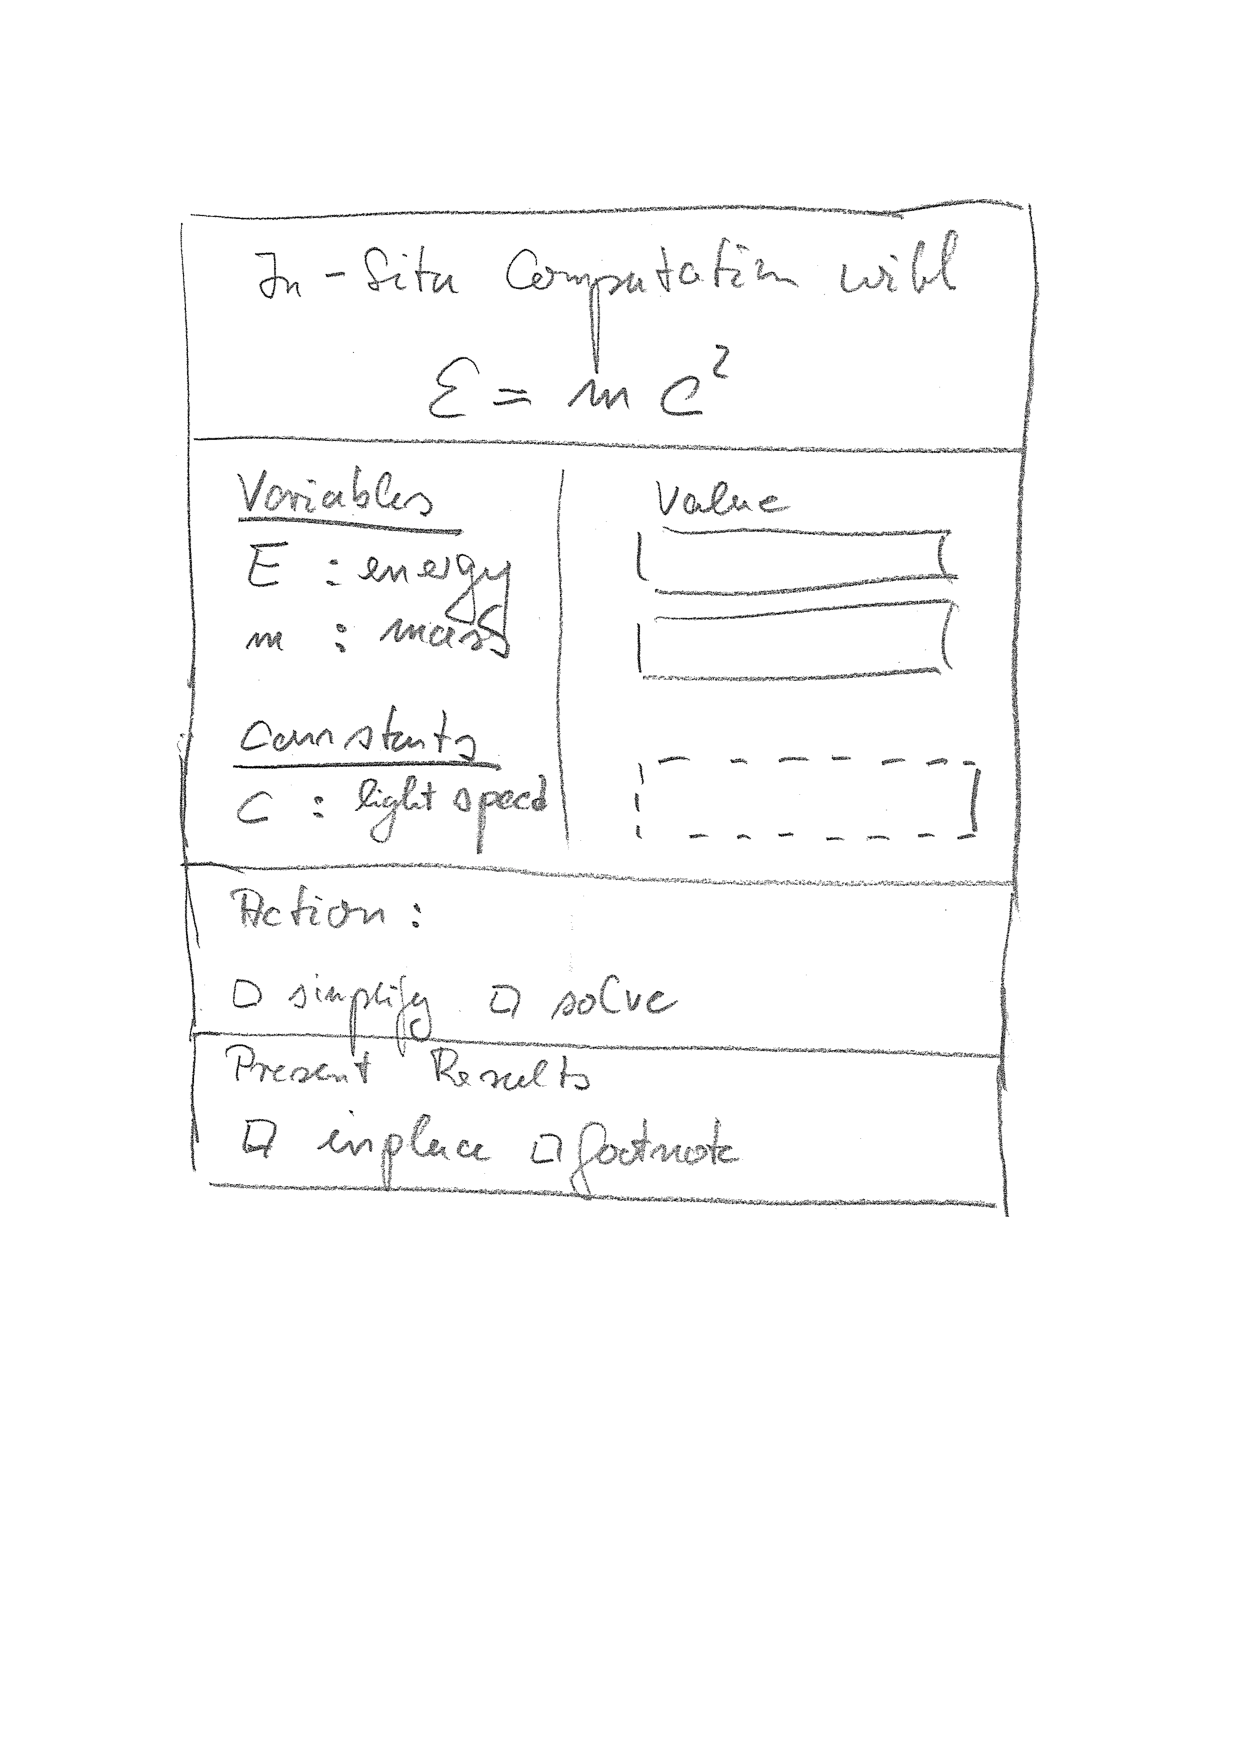
\includegraphics[width=10cm]{compman}
    \caption{In-Situ Computation Manager}\label{fig:compman}
  \end{figure}
\end{newpart}

%%% Local Variables:
%%% mode: latex
%%% TeX-master: "report"
%%% End:
